\documentclass[11pt]{article}
\usepackage[margin=0.75in]{geometry}
\usepackage{graphicx}
\usepackage{amsmath}
\usepackage{hyperref}
\usepackage{enumitem}
\usepackage{tikz}
\usepackage{xcolor}
\usepackage{listings}
\usetikzlibrary{shapes,arrows,positioning,fit,backgrounds}

\definecolor{codegreen}{rgb}{0,0.6,0}
\definecolor{codegray}{rgb}{0.5,0.5,0.5}
\definecolor{codepurple}{rgb}{0.58,0,0.82}
\definecolor{backcolour}{rgb}{0.95,0.95,0.92}

\lstdefinestyle{mystyle}{
    backgroundcolor=\color{backcolour},
    basicstyle=\ttfamily\tiny,
    breakatwhitespace=false,
    breaklines=true,
    captionpos=b,
    keepspaces=true,
    numbers=left,
    numbersep=5pt,
    showspaces=false,
    showstringspaces=false,
    showtabs=false,
    tabsize=2
}

\lstset{style=mystyle}

\title{\textbf{Solstice: End-to-End Pipeline for Medical Document Fact-Checking}}
\author{From PDF Ingestion to Multi-Agent Verification}
\date{}

\begin{document}
\maketitle

\section{Introduction}

Solstice is an AI-native system that transforms unstructured medical PDFs into fact-checked, evidence-backed documents. The pipeline combines computer vision for layout understanding, natural language processing for text extraction, and orchestrated multi-agent systems for claim verification.

\section{Stage 1: PDF Document Ingestion}

\subsection{Layout Detection with Detectron2}

The pipeline begins with sophisticated layout analysis using Detectron2, a state-of-the-art object detection framework. Below is an actual example from a scientific paper processed through our pipeline:

\begin{figure}[htbp]
\centering
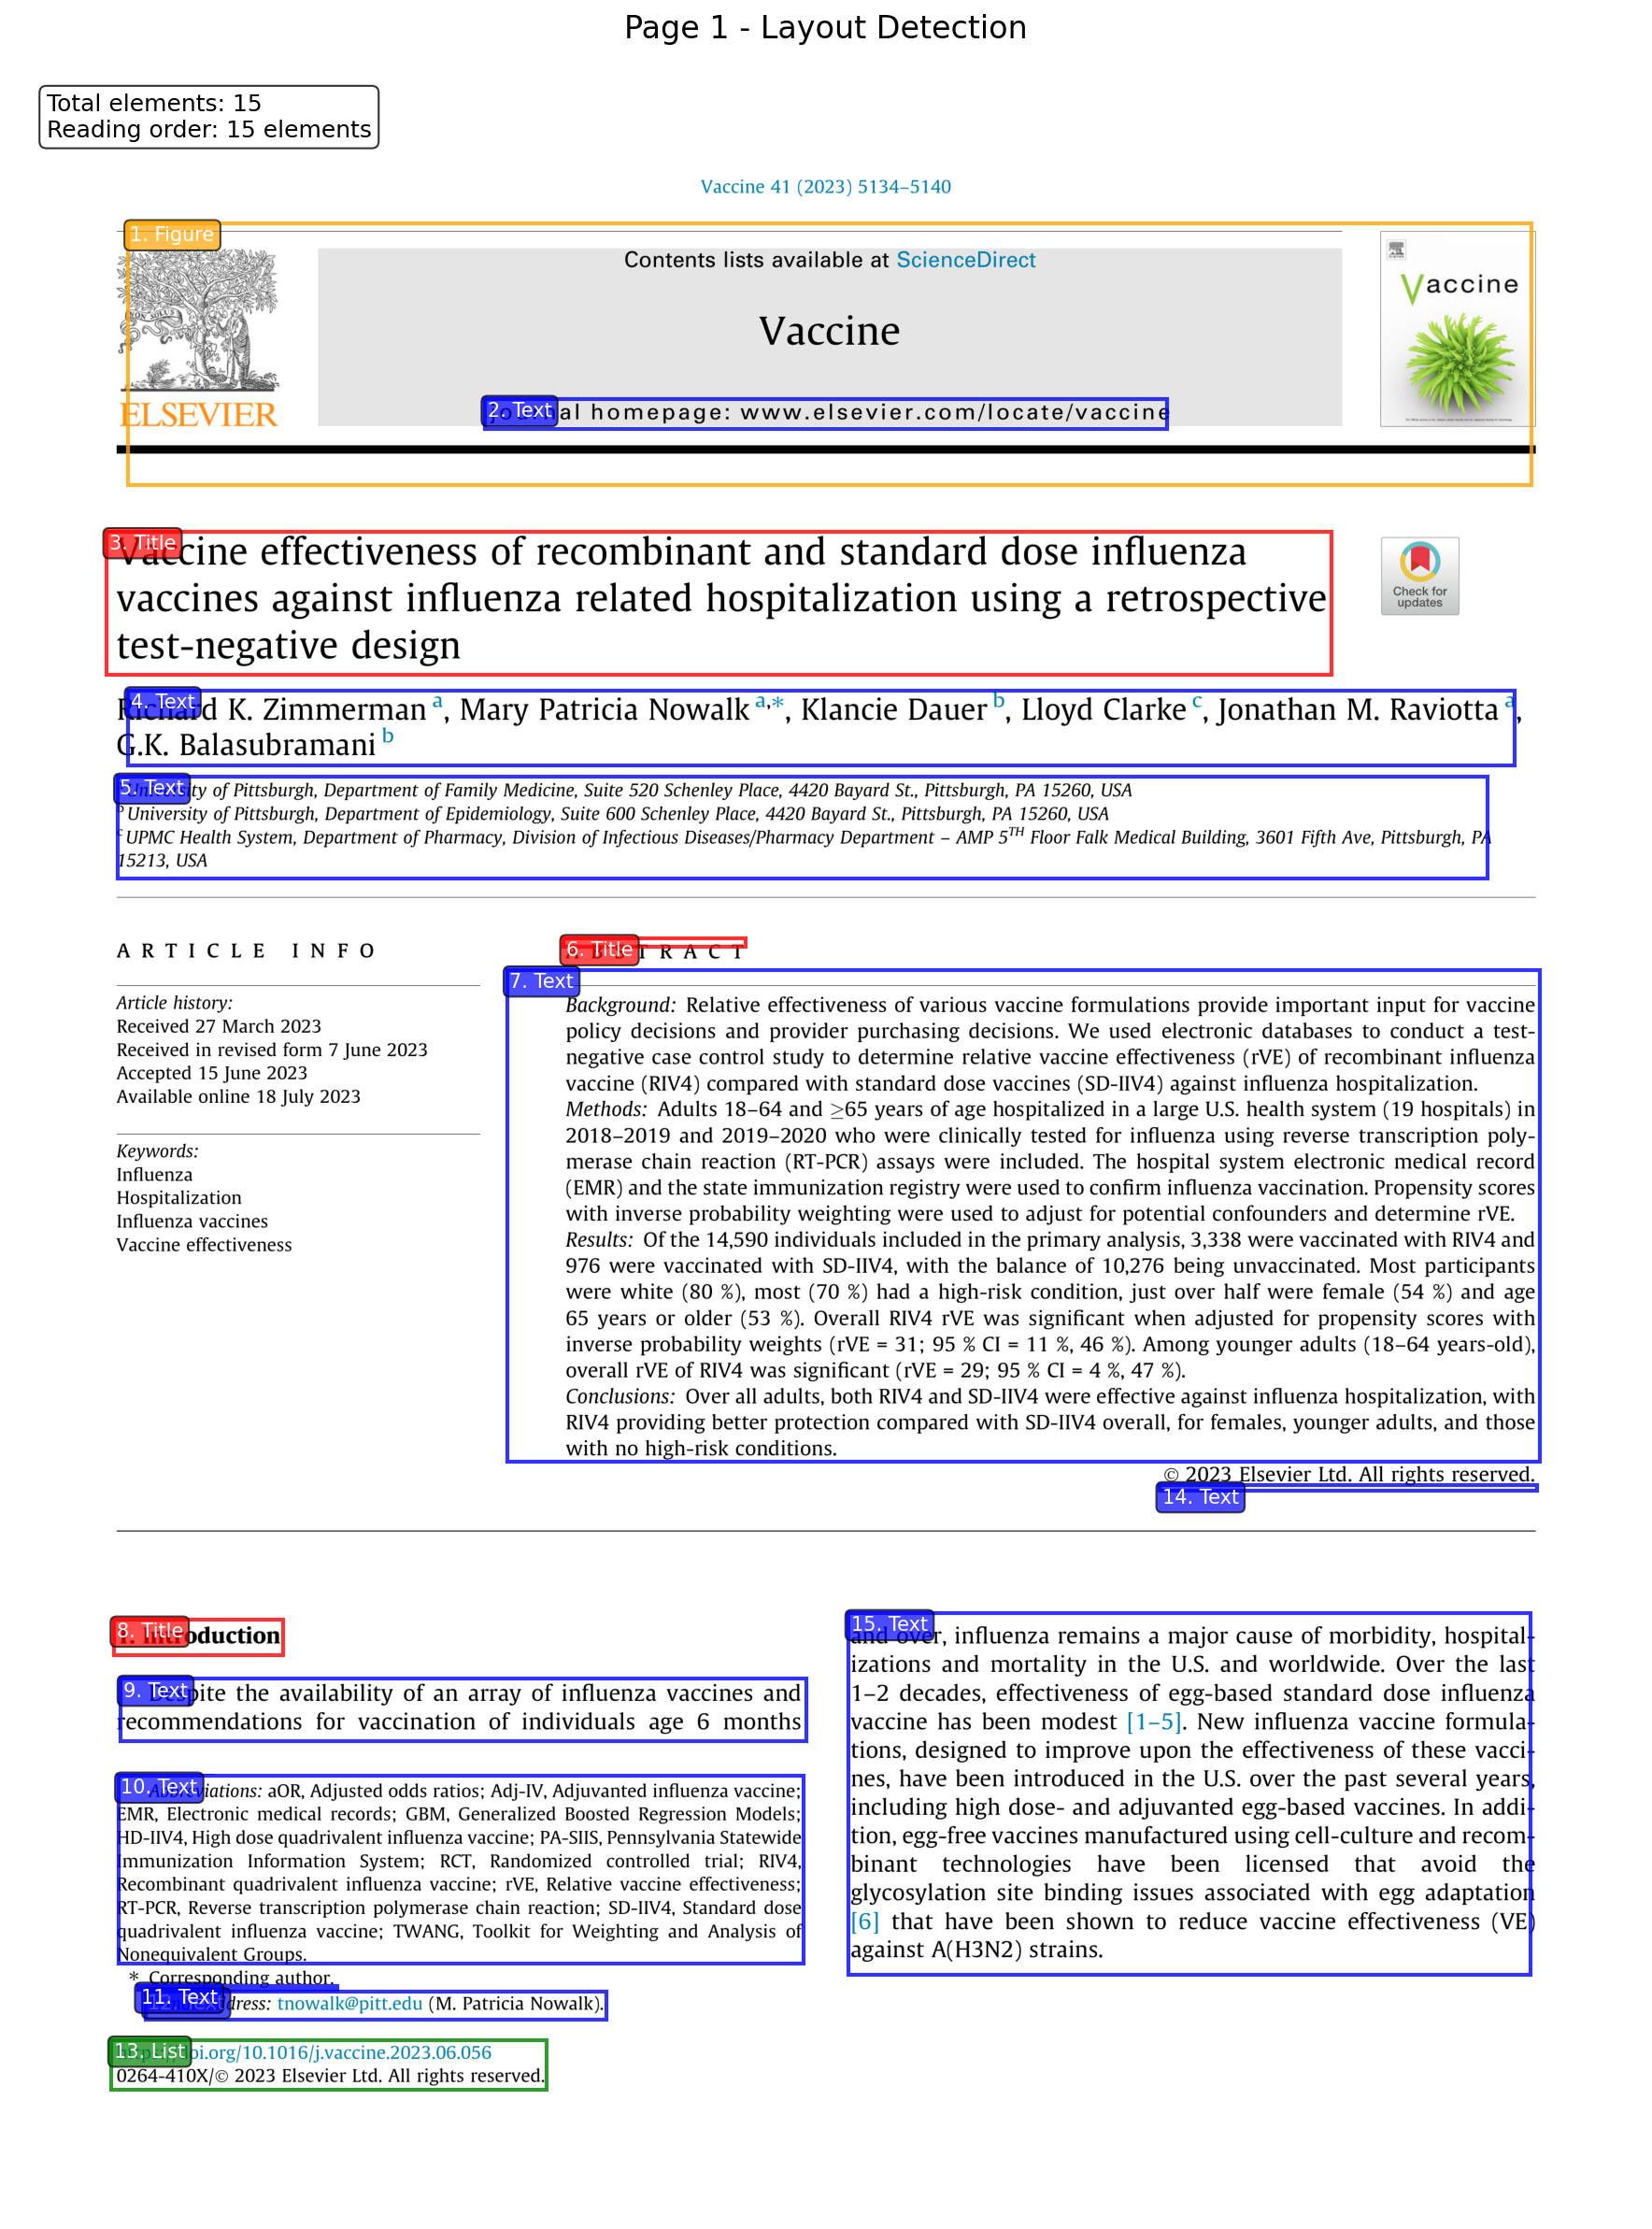
\includegraphics[width=0.8\textwidth]{scientific_layout_example.png}
\caption{Real layout detection output from Zimmerman et al. (2023) showing detected text blocks, tables, and figures with bounding boxes and confidence scores}
\end{figure}

The detection process uses:
\begin{itemize}[leftmargin=*,topsep=0pt,itemsep=0pt]
\item Faster R-CNN with ResNet-50 backbone
\item IoU threshold of 0.7 for overlap resolution
\item Hierarchical nesting for complex layouts
\item Custom post-processing for medical documents
\end{itemize}

\subsection{Text and Visual Extraction}

After layout detection, the pipeline extracts content:

\begin{enumerate}[leftmargin=*,topsep=0pt,itemsep=0pt]
\item \textbf{Text Extraction}: PyMuPDF extracts text within bounding boxes
\item \textbf{OCR Correction}: SymSpell fixes common OCR errors (0→O, l→I)
\item \textbf{Figure/Table Export}: Visual elements saved as 300 DPI PNGs
\item \textbf{Reading Order}: Column detection determines logical flow
\end{enumerate}

\section{Stage 2: Multi-Agent Fact-Checking}

\subsection{Agent Architecture}

The fact-checking system employs specialized agents in an orchestrated pipeline:

\begin{figure}[htbp]
\centering
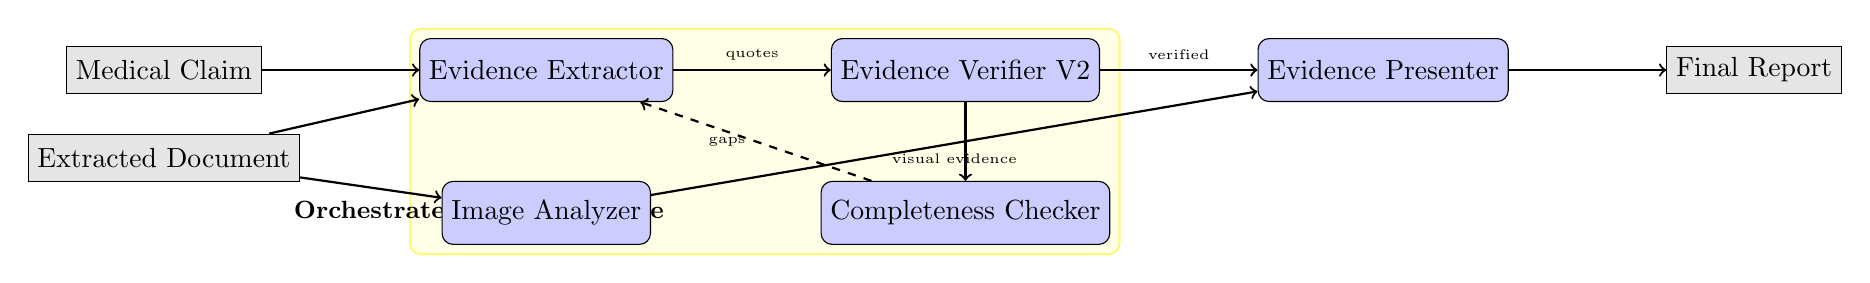
\begin{tikzpicture}[
    node distance=1.5cm,
    agent/.style={rectangle, draw, fill=blue!20, minimum width=2.5cm, minimum height=0.8cm, rounded corners},
    data/.style={rectangle, draw, fill=gray!20, minimum width=2cm, minimum height=0.6cm},
    arrow/.style={->,thick},
    dasharrow/.style={->,thick,dashed}
]

% Input
\node[data] (claim) {Medical Claim};
\node[data, below=0.5cm of claim] (doc) {Extracted Document};

% Agents
\node[agent, right=2cm of claim] (extractor) {Evidence Extractor};
\node[agent, right=2cm of extractor] (verifier) {Evidence Verifier V2};
\node[agent, below=1cm of verifier] (completeness) {Completeness Checker};
\node[agent, right=2cm of verifier] (presenter) {Evidence Presenter};
\node[agent, below=1cm of extractor] (image) {Image Analyzer};

% Outputs
\node[data, right=2cm of presenter] (report) {Final Report};

% Connections
\draw[arrow] (claim) -- (extractor);
\draw[arrow] (doc) -- (extractor);
\draw[arrow] (extractor) -- node[above] {\tiny quotes} (verifier);
\draw[arrow] (verifier) -- node[above] {\tiny verified} (presenter);
\draw[arrow] (verifier) -- (completeness);
\draw[dasharrow] (completeness) -- node[left] {\tiny gaps} (extractor);
\draw[arrow] (doc) -- (image);
\draw[arrow] (image) -- node[below] {\tiny visual evidence} (presenter);
\draw[arrow] (presenter) -- (report);

% Background boxes
\begin{pgfonlayer}{background}
\node[fit=(extractor)(verifier)(completeness)(image), fill=yellow!10, draw=yellow!50, thick, rounded corners] {};
\node at (4,-1.8) {\small \textbf{Orchestrated Agent Pipeline}};
\end{pgfonlayer}

\end{tikzpicture}
\caption{Multi-agent system architecture with feedback loops for comprehensive evidence extraction}
\end{figure}

\subsection{Agent Responsibilities}

\subsubsection{Evidence Extractor}
\begin{lstlisting}[language=Python]
# Searches for claim-relevant quotes
async def extract_evidence(claim, document):
    model = "gpt-4"
    temperature = 0  # Deterministic
    
    quotes = search_document(claim, document)
    return preserve_exact_quotes(quotes)
\end{lstlisting}

\subsubsection{Evidence Verifier V2}
Validates that extracted quotes exist in the source:
\begin{itemize}[leftmargin=*,topsep=0pt,itemsep=0pt]
\item Semantic matching for OCR variations
\item Filters tangential content
\item Returns verification statistics
\end{itemize}

\subsubsection{Completeness Checker}
Identifies gaps and triggers additional extraction:
\begin{itemize}[leftmargin=*,topsep=0pt,itemsep=0pt]
\item Reviews verified evidence coverage
\item Searches for missing aspects
\item Feeds findings back to pipeline
\end{itemize}

\subsubsection{Image Evidence Analyzer}
Processes visual elements with vision models:
\begin{lstlisting}[language=Python]
# Analyzes figures and tables
async def analyze_image(image_path, claim):
    model = "claude-3"  # Multimodal
    
    analysis = await model.analyze(
        image=load_image(image_path),
        claim=claim
    )
    return {
        "supports_claim": analysis.relevant,
        "explanation": analysis.details
    }
\end{lstlisting}

\section{Stage 3: Output Generation}

\subsection{Evidence Presentation}

The final stage consolidates all evidence into structured outputs:

\begin{enumerate}[leftmargin=*,topsep=0pt,itemsep=0pt]
\item \textbf{JSON Output}: Machine-readable evidence with metadata
\item \textbf{HTML Reports}: Human-readable with embedded images
\item \textbf{Coverage Assessment}: Complete/partial/none ratings
\item \textbf{Confidence Scores}: Based on evidence quantity/quality
\end{enumerate}

\subsection{Marketing Material Processing}

The system includes a specialized pipeline for marketing materials with enhanced visual element detection:

\begin{figure}[htbp]
\centering
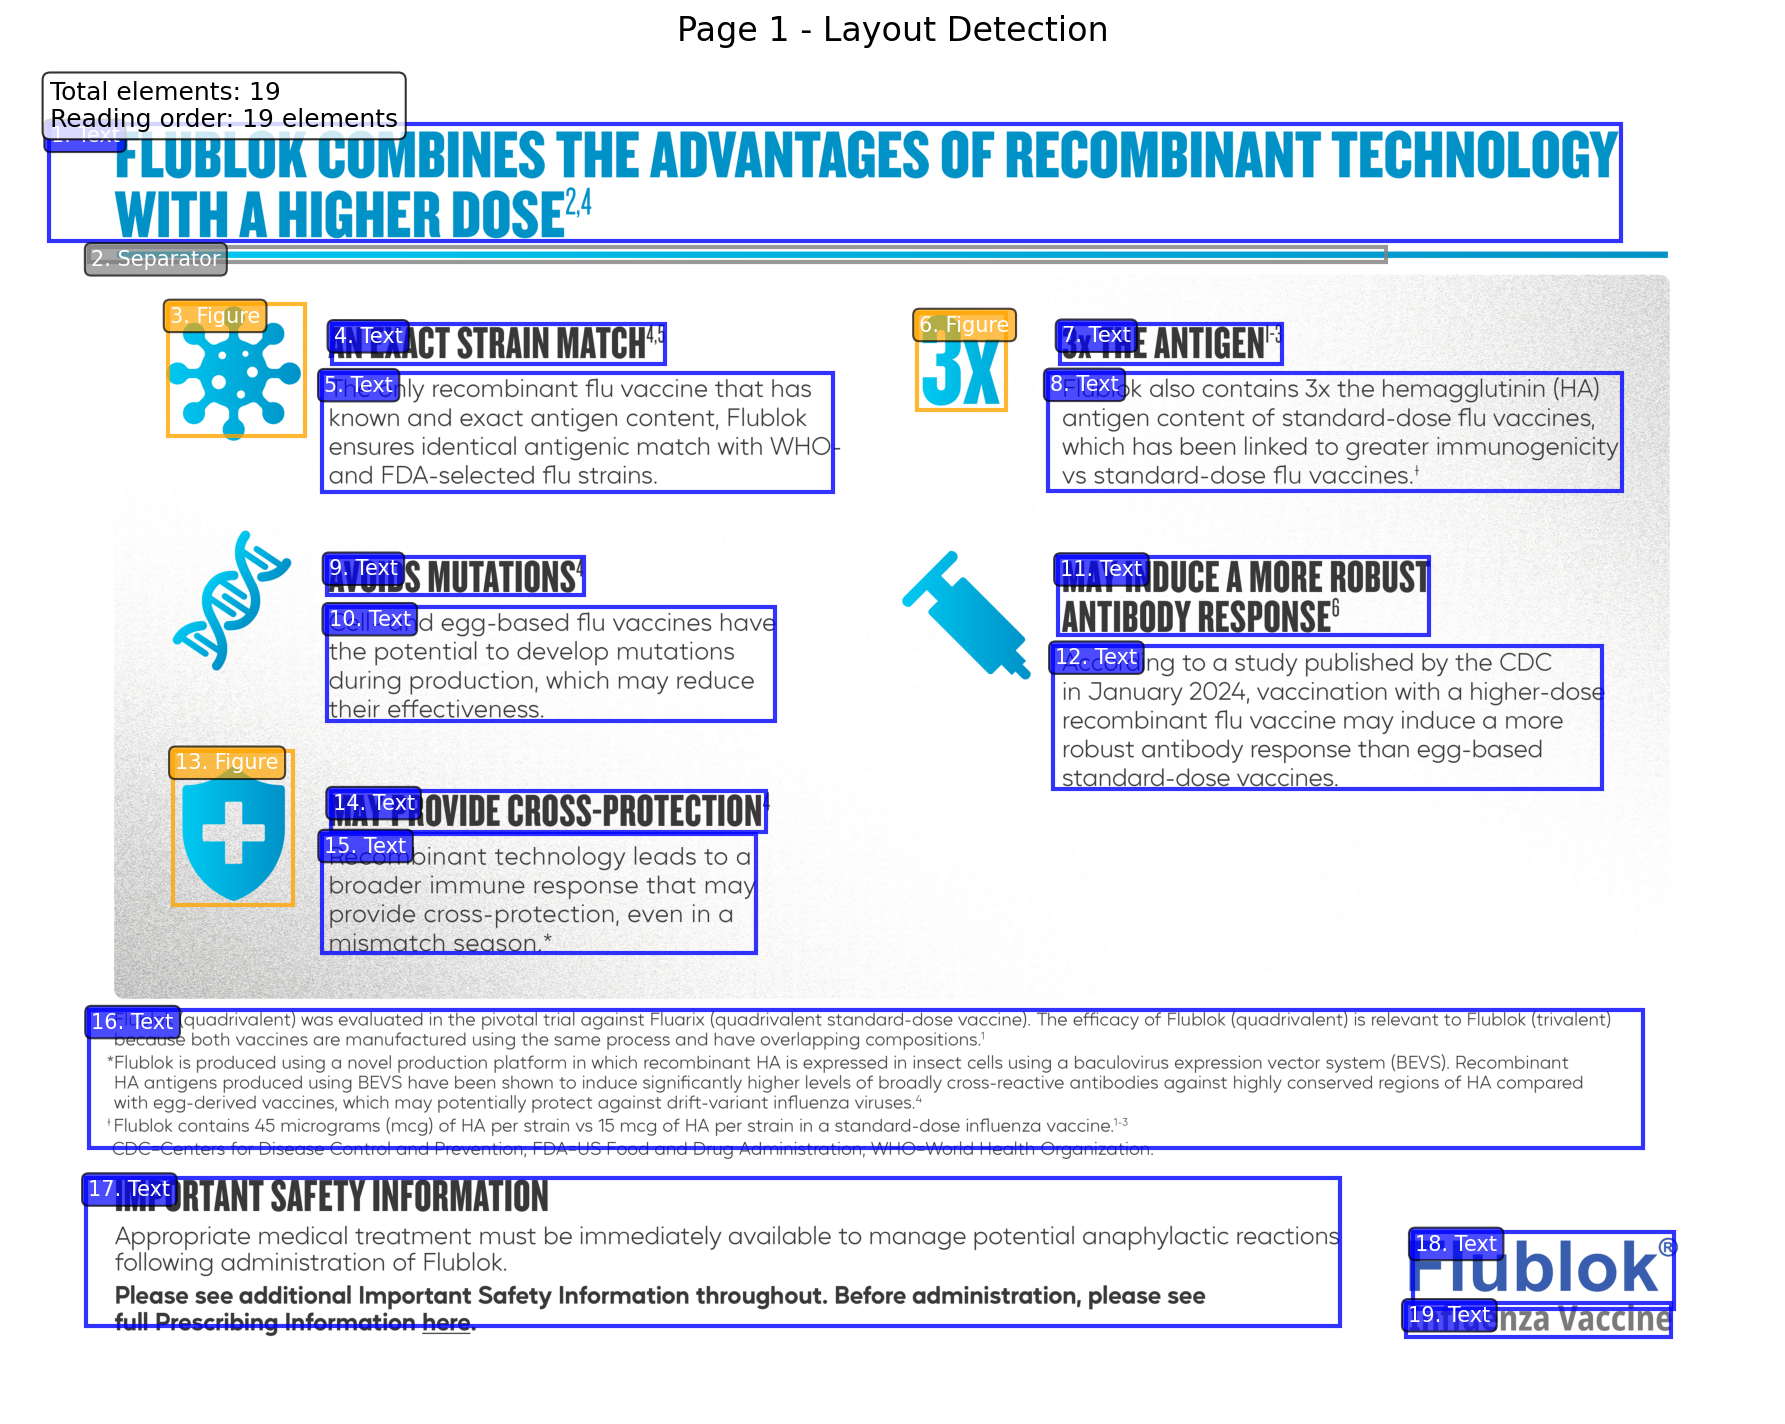
\includegraphics[width=0.8\textwidth]{marketing_layout_example.png}
\caption{Marketing material layout detection from Flublok one-pager showing detection of promotional graphics, key benefit callouts, and visual hierarchy elements}
\end{figure}

Marketing pipeline differences:
\begin{itemize}[leftmargin=*,topsep=0pt,itemsep=0pt]
\item Separate cache directory (data/marketing\_cache/)
\item Enhanced visual element extraction
\item Claim detection from promotional language
\item Cross-referencing with clinical evidence
\end{itemize}

\section{Implementation Details}

\subsection{Orchestration and Parallelism}

\begin{lstlisting}[language=Python]
# Parallel claim processing with semaphore
async def process_claims(claims, documents):
    semaphore = asyncio.Semaphore(2)
    
    async def process_single(claim):
        async with semaphore:
            return await claim_orchestrator.run(
                claim, documents
            )
    
    results = await asyncio.gather(*[
        process_single(c) for c in claims
    ])
    return results
\end{lstlisting}

\subsection{Error Handling and Reliability}

\begin{itemize}[leftmargin=*,topsep=0pt,itemsep=0pt]
\item \textbf{Retry Logic}: Exponential backoff for API failures
\item \textbf{JSON Parsing}: Handles markdown-wrapped responses
\item \textbf{Token Management}: Dynamic adjustment for long documents
\item \textbf{Cache System}: All intermediate results persisted
\end{itemize}

\section{Real-World Applications}

Current deployments include:
\begin{enumerate}[leftmargin=*,topsep=0pt,itemsep=0pt]
\item \textbf{Vaccine Studies}: Efficacy claims vs clinical trials
\item \textbf{Drug Safety}: Package inserts vs FDA documents
\item \textbf{Medical Devices}: Marketing claims vs regulatory filings
\item \textbf{Treatment Guidelines}: Recommendations vs evidence base
\end{enumerate}

\section{Performance Characteristics}

\begin{itemize}[leftmargin=*,topsep=0pt,itemsep=0pt]
\item \textbf{Layout Detection}: 95\%+ mAP on medical PDFs
\item \textbf{Text Extraction}: 99\%+ accuracy with OCR correction
\item \textbf{Evidence Verification}: 80-90\% verification rates
\item \textbf{Processing Speed}: 2-3x speedup with parallelization
\item \textbf{Image Analysis}: 30-40\% of images contain relevant evidence
\end{itemize}

\section{Conclusion}

Solstice demonstrates how modern AI capabilities can be orchestrated to solve complex document processing challenges. By combining layout understanding, multimodal analysis, and agent-based verification, the system provides reliable fact-checking for medical documentation while maintaining full traceability through comprehensive caching.

\end{document}